\documentclass[a4paper,12pt]{article}
\usepackage[utf8]{inputenc}

\usepackage[brazil]{babel}
\usepackage[lmargin=3cm,tmargin=3cm,rmargin=2cm,bmargin=2cm]{geometry}
\usepackage[T1]{fontenc}
\usepackage{amsmath,amsthm,amsfonts,amssymb,dsfont,mathtools}
\usepackage{blindtext}
\usepackage{graphicx} % Required for inserting images
\usepackage{listings}
\usepackage{xcolor}

\definecolor{codegreen}{rgb}{0,0.6,0}
\definecolor{codegray}{rgb}{0.5,0.5,0.5}
\definecolor{codepurple}{rgb}{0.8,0,0.2}
\definecolor{backcolour}{rgb}{.95,.95,1}
\definecolor{backcolour2}{rgb}{255,255,255}

\lstdefinestyle{mystyle}{
    backgroundcolor=\color{backcolour},   
    commentstyle=\color{codegreen},
    keywordstyle=\color{blue},
    numberstyle=\tiny\color{codegray},
    stringstyle=\color{codepurple},
    basicstyle=\ttfamily\footnotesize,
    breakatwhitespace=false,         
    breaklines=true,                 
    captionpos=b,                    
    keepspaces=true,                 
    numbers=left,                    
    numbersep=5pt,                  
    showspaces=false,                
    showstringspaces=false,
    showtabs=false,                  
    tabsize=2
}
\lstdefinestyle{mystyle2}{
    backgroundcolor=\color{backcolour2},   
    commentstyle=\color{red},
    keywordstyle=\color{blue},
    numberstyle=\tiny\color{black},
    stringstyle=\color{purple},
    basicstyle=\ttfamily\small,
    breakatwhitespace=false,         
    breaklines=true,                 
    captionpos=b,                    
    keepspaces=true,                 
    numbers=none,                    
    numbersep=5pt,                  
    showspaces=false,                
    showstringspaces=false,
    showtabs=false,                  
    tabsize=2
}
\lstset{style=mystyle,mystyle2}
\begin{document}


\begin{center}
\textbf{FATEC RUBENS LARA}

\textbf{CURSO DE CIÊNCIA DE DADOS}

\vspace{3cm}

\textbf{RELATÓRIO DE MATEMÁTICA: FORMULA DE LEIBNIZ}

\vspace{3cm}

\textbf{GUSTAVO MIRANDA SILVA ARAÚJO}

\textbf{GUSTAVO FERREIRA GONÇALVES LIMA}

\vfill

\begin{flushright}
Santos - São Paulo\\
11/05/2023
\end{flushright}
\end{center}

\begin{figure}{}
\centering
\label{}

\includegraphics[width=14cm,height=2cm]{rodap-4.png}
\end{figure}

\clearpage



\begin{figure}
1) Deduza A o determinate 4x4 usando a formula:\\\\\\
    \centering
    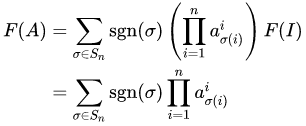
\includegraphics[height=4cm]{leibniz.png}
    \caption{Formula de leibniz}
    \label{fig:my_label}
\end{figure}

Todas as permutações do Conjunto S de índice n = 4

\begin{center}
\begin{lstlisting}[style=mystyle2]
{1,2,3,4}, {1,2,4,3}, {1,3,2,4}, {1,3,4,2}, {1,4,2,3}, {1,4,3,2}
{2,1,3,4}, {2,1,4,3}, {2,3,1,4}, {2,3,4,1}, {2,4,1,3}, {2,4,3,1}
{3,1,2,4}, {3,1,4,2}, {3,2,1,4}, {3,2,4,1}, {3,4,1,2}, {3,4,2,1}
{4,1,2,3}, {4,1,3,2}, {4,2,1,3}, {4,2,3,1}, {4,3,1,2}, {4,3,2,1} \end{lstlisting}
\end{center}
A =
$
\left[\begin{array}{cccc}
	a11 & a12 & a13 & a14\\
	a21 & a22 & a23 & a24\\
	a31 & a32 & a33 & a34\\
    a41 & a42 & a43 & a44\\
\end{array}\right]
\\
$
\\\\
det (A) = \\\\
$
   a11 * a22 * a33 * a44  +  a11 * a23 * a34 * a42  +  a11 * a24 * a32
* a43\\
+  a12 * a21 * a34 * a43  +  a12 * a23 * a31 * a44  +  a12 * a24 *
a33 * a41\\
+  a13 * a21 * a32 * a44  +  a13 * a22 * a34 * a41 + a13 * a24 *
a31 * a42\\
+  a14 * a21 * a33 * a42  +  a14 * a22 * a31 * a43  +  a14 * a23 *
a32 * a41\\
-  a11 * a22 * a34 * a43  -  a11 * a23 * a32 * a44  -  a11 * a24 *
a33 * a42\\
-  a12 * a21 * a33 * a44  -  a12 * a23 * a34 * a41  -  a12 * a24 *
a31 * a43\\
-  a13 * a21 * a34 * a42  -  a13 * a22 * a31 * a44  -  a13 * a24 *
a32 * a41\\
-  a14 * a21 * a32 * a43  -  a14 * a22 * a33 * a41 - a14 * a23 *
a31 * a42 
$
\pagebreak
\\\\ 

2) Calcule o determiante, usando o que foi deduzido, de duas matrizes definida por:
\\\\
    det(A) = 0 e det(A) != 0
\\\\
A1 =
$
\left[\begin{array}{cccc}
	4 & 8 & 12 & 16\\
	5 & 10 & 15 & 20\\
	6 & 12 & 18 & 24\\
    -15 & -30 & -35 & -60\\
\end{array}\right]
$
\\\\\\
$
4*10*18*(-60)-4*10*24*(-35)-4*15*12*(-60)+4*15*24*(-30)\\+4*20*12*(-35)-4*20*18*(-30)-8*5*18*(-60)+8*5*24*(-35)+8*15*6*(-60)\\-8*15*24*(-15)-8*20*6*(-35)+8*20*18*(-15)+12*5*12*(-60)-12*5*24*(-30)\\-12*10*6*(-60)+12*10*24*(-15)+12*20*6*(-30)-12*20*12*(-15)-16*5*12*(-35)\\+16*5*18*(-30)+16*10*6*(-35)-16*10*18*(-15)-16*15*6*(-30)\\+16*15*12*(-15)
=
0
$
\\\\
det(A) = 0
\\\\
A2 =
$
\left[\begin{array}{cccc}
	5 & -3 & 0 & 4\\
   -3 & 6 & 3 & -3\\
    0 & 3 & 2 & 1\\
    4 & -3 & 1 & 7\\
\end{array}\right]
$
\\\\\\
$
5*6*2*7-5*6*1*1-5*3*3*7+5*3*1*(-3)+5*(-3)*3*1-5*(-3)*2*(-3)--3*(-3)*2*7+-3*(-3)*1*1+-3*3*0*7--3*3*1*4--3*(-3)*0*1+-3*(-3)*2*4+0*(-3)*3*7-4*(-3)*3*1+4*(-3)*2*(-3)+4*6*0*1-4*6*2*4-4*3*0*(-3)+4*3*3*4
=
-54
$
\\\\
det(A) = -54
\pagebreak

3) Programar o método em python, verifique o resultado:

\begin{lstlisting}[language=python, caption=Código referente ao cálculo de determinantes]
n = 4
matriz = []
for i in range(n):
    linha = []
    for j in range(n):
        valor = int(input(f"Digite o valor da posicao [{i+1}][{j+1}]: "))
        linha.append(valor)
    matriz.append(linha)

def leibniz(matriz):
    n = len(matriz)
    if n == 1:
        return matriz[0][0]
    else:
        soma = 0
        for j in range(n):
            nova_matriz = []
            for i in range(1, n):
                linha = []
                for k in range(n):
                    if k != j:
                        linha.append(matriz[i][k])
                nova_matriz.append(linha)
            sinal = (-1) ** j
            soma += matriz[0][j] * sinal * leibniz(nova_matriz)
        return soma

deta = leibniz(matriz)
print("O determinante da matriz:",deta)
\end{lstlisting}
\pagebreak

A =
$
\left[\begin{array}{cccc}
	4 & 8 & 12 & 16\\
	5 & 10 & 15 & 20\\
	6 & 12 & 18 & 24\\
    -15 & -30 & -35 & -60\\
\end{array}\right]
$
\begin{figure}[h]
Matriz tendo seu determinante calculado em python:\\\\\\
    \centering
    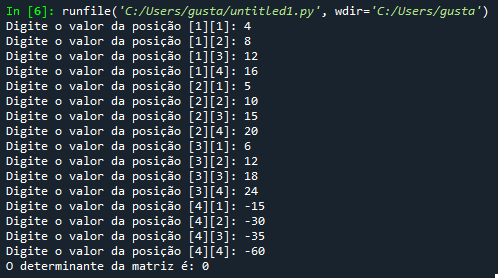
\includegraphics[height=10cm,width=15cm]{console1.png}
    \caption{Console do python}
    \label{fig:my_label}
\end{figure}

\pagebreak
A =
$
\left[\begin{array}{cccc}
	5 & -3 & 0 & 4\\
   -3 & 6 & 3 & -3\\
    0 & 3 & 2 & 1\\
    4 & -3 & 1 & 7\\
\end{array}\right]
$
\\
\begin{figure}[h]
Matriz tendo seu determinante calculado em python:\\\\\\
    \centering
    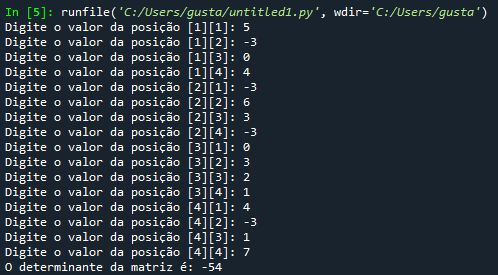
\includegraphics[height=10cm,width=15cm]{console2.png}
    \caption{Console do python}
    \label{fig:my_label}
\end{figure}



\end{document}


